\chapter{Dokumentácia}

\section{Inštalácia}
\subsection{Požiadavky}
Aplikácia vyžaduje aby na každej stanici bol nainštalovaný .NET framework verzia 4.5, v ktorom je aplikácia vyvíjaná. Ďalej aplikácia potrebuje aby stanica pomocou sieťovej komunikácie dokázala kontaktovať server, z ktorého bude sťahovať balíky. Tento server musí mať zložku s balíkmi prístupnú cez HTTP protokol a zároveň musí mať nainštalovaný SSL certifikát, pomocou ktorého sa bude identifikovať používateľovi pri požiadavke na stiahnutie balíku.

\subsection{Detailný postup inštalácie}
V tejto sekcii dôkladne popíšeme postup, ktorým uvedieme aplikáciu do funkčného stavu.
\begin{enumerate}
\item Z priloženého CD skopírujeme alebo stiahneme z internetu súbor SetItUp.zip
\item Tento súbor rozbalíme do zložky, kde chceme mať našu aplikáciu nainštalovanú
\item S administrátorskými právami spustíme UserApp.exe a vyplníme cesty k významným priečinkom - priečinok s balíkmi, priečinok s odkazmi, adresa vzdialeného serveru
\item Spustíme SetItUpService.exe s argumentom install, ktorý nám do systému nainštaluje potrebnú službu. Taktiež vyžaduje administrátorské práva
\item Následne spustíme Administration.exe a môžme začať monitorovať inštalácie programov
\item Po každom vytvorenom balíku odkopírujeme súbor packages.txt a \textless názov balíku\textgreater.zip na server. Súbor packages.txt obsahuje všetky balíky, ktoré boli zapísané na serveri pri spustení aplikácie nasledované balíkmi, ktoré sme vytvorili v rámci tejto inštancie aplikácie.
\end{enumerate}

\section{Konfigurácia}
Aplikácia si k správnemu behu potrebuje nakonfigurovať cesty k dôležitým priečinkom ako je priečinok s balíčkami, s odkazmi a adresa serveru na ktorom sú uložené balíky. Táto konfigurácia prebehne pri prvom spustení aplikácie pomocou UserApp.exe, ktorá si vypýta cesty k týmto zložkám. Program taktiež udržuje dôležité informácie o balíčkoch v 3 konfiguračných súboroch. Zároveň existuje štvrtý konfiguračný súbor, ktorý nesie informáciu o slovách, ktoré ignorujeme pri tvorbe balíku.

\subsection{packages.txt}
Tento súbor je uložený na serveri a obsahuje zoznam všetkých balíčkov. Kópie na používateľských počítačoch sa pri každom spustení služby alebo aplikácie Administration nahradia tou zo serveru. V tomto súbore sú zapísané aj odkazy na balíčky, ktoré sa majú vytvoriť a cesta k spustiteľnému súboru v prípade, že balíček je nainštalovaný. Odkazy sú zapísané pri zozname balíčkov, aby služba, ktorá sa stará o vytváranie odkazov, nemusela rozbaľovať všetky balíky. V súbore namiesto medzier používame znaky \textasciitilde\textasciitilde, aby sme vedeli rozlíšiť medzery vytvorené našim programom a medzery v názve súboru alebo priečinku.
\begin{listing}
\begin{minted}[mathescape,
               linenos,
               numbersep=5pt,
               frame=lines,
               framesep=2mm]{text}  
pm~~PowerISO
s~~PowerISO~~D:\Bakalar\Power ISO\PowerISO.exe
pa~~netFramework
\end{minted}
\caption{Štruktúra packages.txt}
\label{lst:pack}
\end{listing}
V prvom riadku máme písmeno P ako identifikátor riadku s názvom balíku a následne samotný názov balíku. Písmeno M alebo A, ktoré sa nachádza na druhom mieste, označuje či je balík nainštalovaný na vyžiadanie alebo automaticky pri štarte systému. Po tomto riadku nasledujú riadky označené písmenom S, ktoré popisujú aké odkazy majú byť vytvorené k danému balíku. Ako prvý je zadaný názov odkazu, ktorý sa ma vytvoriť a za ním je zapísaná cesta k spustiteľnému súboru reprezentovanému týmto odkazom.
\begin{figure}[h]
    \centering
    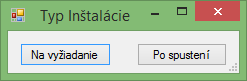
\includegraphics[width=0.5\textwidth]{installtype}
    \caption{Výber typu inštalácie}
    \label{fig:installtype}
\end{figure}

\subsection{depedencies.txt}
V tomto súbore, ktorý sa nachádza v každom balíku zvlášť, sú zapísané informácie o balíkoch, ktoré musia byť nainštalované spolu s daným balíkom. Jeho štruktúra je jednoduchá, na každom riadku je 1 názov balíku, ktorý musí byť nainštalovaný.
\begin{figure}[h]
    \centering
    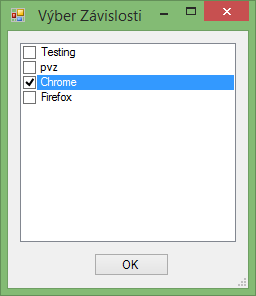
\includegraphics[width=0.5\textwidth]{depend}
    \caption{Výber závislostí}
    \label{fig:depend}
\end{figure}

\subsection{\textless názov balíku\textgreater.txt}
Je to hlavný súbor v balíku, ktorý v sebe drží informácie o miestach kam majú byť súbory prenesené. Jeho štruktúra je taktiež jednoduchá, na každom riadku si pamätá cestu k jednému súboru. Keď z tejto cesty odoberieme názov disku, dostaneme relatívnu cestu k danému súboru v zložke balíku.

\subsection{blacklist.txt}
Je súbor, ktorý sa nachádza lokálne v zložke s balíkmi, potrebný pri vytváraní balíkov. V ňom nájdeme zoznam slov, ktorých výskyt v ceste k súboru spôsobí, že daný súbor nebude zapísaný medzi súbory daného balíku. V momente kontroly týchto slov sa všetko zmení na malé písmena, preto aj v tomto konfiguračnom súbore je všetko zapísané malými písmenami.

\subsection{Registre}
Počas tvorby balíku aplikácia kontroluje zmeny vo Windows registroch v podstrome \textit{HKEY\textunderscore LOCAL\textunderscore MACHINE/SOFTWARE/}, všetky zmeny budú zapísané v súboroch v priečinku SetItUp_Registry uloženom v balíku. Takisto monitorujeme \textit{HKEY\textunderscore CURRENT\textunderscore USER/SOFTWARE/}, avšak s tieto registre neskôr pri inštalácií nepoužívame, sú tam pripravené pre potreby administrátora. Naša aplikácia si cesty k dôležitým priečinkom pamätá v kľúči \textit{HKEY\textunderscore LOCAL\textunderscore MACHINE/SOFTWARE/SetItUp}.

\section{Spúšťanie}
\subsection{Administrátor}
Po nainštalovaní aplikácie spustí UserApp.exe a SetItUpService.exe aby nakonfiguroval aplikácie a pripravil službu, ktorá sa stará o aktualizáciu zoznamu balíkov a odkazov. Následne bude pomocou Administration.exe vytvárať balíky, ktoré budú neskôr prístupné používateľovi.

\subsection{Používateľ}
V ponuke Štart bude mať špeciálne odkazy na programy, pomocou ktorých sa mu daná program nainštaluje a následne spustí. Ostatok aplikácie vyžaduje administrátorské práva a preto s ním obyčajný používateľ nebude môcť narábať.
\begin{figure}[h]
    \centering
    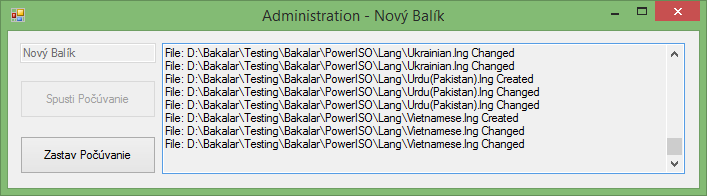
\includegraphics[width=0.8\textwidth]{hlavne}
    \caption{Hlavné okno}
    \label{fig:hlavne}
\end{figure}
\begin{figure}[h]
    \centering
    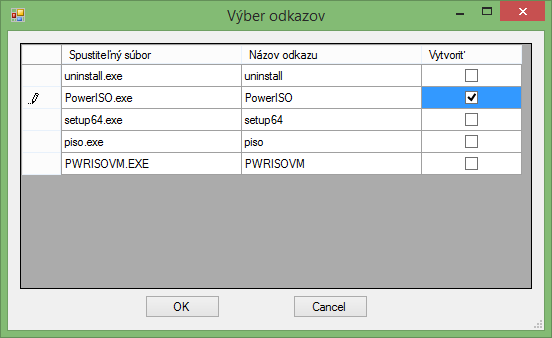
\includegraphics[width=0.8\textwidth]{odkazy}
    \caption{Výber odkazov na vytvorenie}
    \label{fig:links}
\end{figure}

\section{Správa balíkov}
\subsection{Vytvorenie balíku}
Po spustení administrátorskej aplikácie, sa zobrazí rozhranie v ktorom administrátor dokáže spustiť sledovanie inštalácie a kontrolovať v konzole priebeh sledovania a chybové správy. Po skončení sledovania bude prezentovaný formulárom na výber odkazov, ktoré majú byť dostupné používateľovi, výberom balíkov na ktorých je práve vytváraný balík závislý a zvolením kedy má byť balík inštalovaný.

\subsection{Zoznam balíkov}
Zoznam balíkov je zapísaný v súbore na serveri. Lokálne sa tento zoznam aktualizuje pri každom spustení služby a časti aplikácie Administration.exe. Administrátor môže manuálne meniť nastavenia balíkov, zmenou textových súborov v zložke s balíkmi. V týchto konfiguračných súboroch je zapísaný zoznam balíkov, odkazov, ktoré sa majú vytvoriť a zoznam zakázaných slov pri počúvaní. Takisto v zložke s balíkom nájdeme súbory so zoznamom súborov daného balíku a závislosťami, ktoré daný balík má.

\subsection{Inštalácia balíku}
Používateľ môže nainštalovať balík spustením odkazu zo zložky s odkazmi. Tento odkaz zistí, či už je daný balík nainštalovaný a podľa toho sa rozhodne o ďalšom kroku. Ak balík ešte nebol nainštalovaný, aplikácia informuje službu, ktorá nakopíruje potrebné súbory na určené miesto. V prípade, že balík bol nainštalovaný, aplikácia spustí požadovaný program.